\documentclass[14pt,a4paper, oneside]{report}

%%%%%%%%%%%%%%%%%%%%%%%% Шрифты %%%%%%%%%%%%%%%%%%%%%%%%%%%%%%%%%
\usepackage{fontspec}         % пакет для подгрузки шрифтов
\setmainfont{Arial}   % задаёт основной шрифт документа

\usepackage{polyglossia}      % Пакет, который позволяет подгружать русские буквы
\setdefaultlanguage{russian}  % Основной язык документа

\usepackage{float}               % возможность позиционировать объекты в нужном месте

%%%%%%%%%% Работа с картинками %%%%%%%%%
\usepackage{graphicx}                  % Для вставки рисунков
\usepackage{graphics}
                   
%%%%%%%%%% Гиперссылки %%%%%%%%%%
\usepackage{hyperref}
\hypersetup{
     colorlinks=true,       	% true - цветные ссылки, false - ссылки в рамках
     urlcolor=black,          % цвет ссылки на url
 }

%%%% Оформление %%%%%%%
\usepackage{extsizes} % Возможность сделать 14-й шрифт

% размер листа бумаги
\usepackage[paper=a4paper,top=10mm, bottom=10mm,left=35mm,right=35mm,includefoot,includehead]{geometry}

\usepackage{setspace}
\setstretch{1}  % Межстрочный интервал
\setlength{\parindent}{0em} % Красная строка.
\setlength{\parskip}{0.5mm}   % Расстояние между абзацами

\usepackage{fancyhdr} % Колонтитулы
\pagestyle{fancy}

\renewcommand{\headrulewidth}{0.2pt}  % Толщина линий, отчеркивающих верхний
\renewcommand{\footrulewidth}{0pt}  % и нижний колонтитулы
	\rhead{\thepage}
 	\lhead{{\MakeUppercase {\thesection \quad \currentname } }}
	\cfoot{Школа Чародейства и Волшебства «Хогвартс»} 


%волшебная палочка в качестве item 
\renewcommand{\labelitemi}{\textcolor{blue}{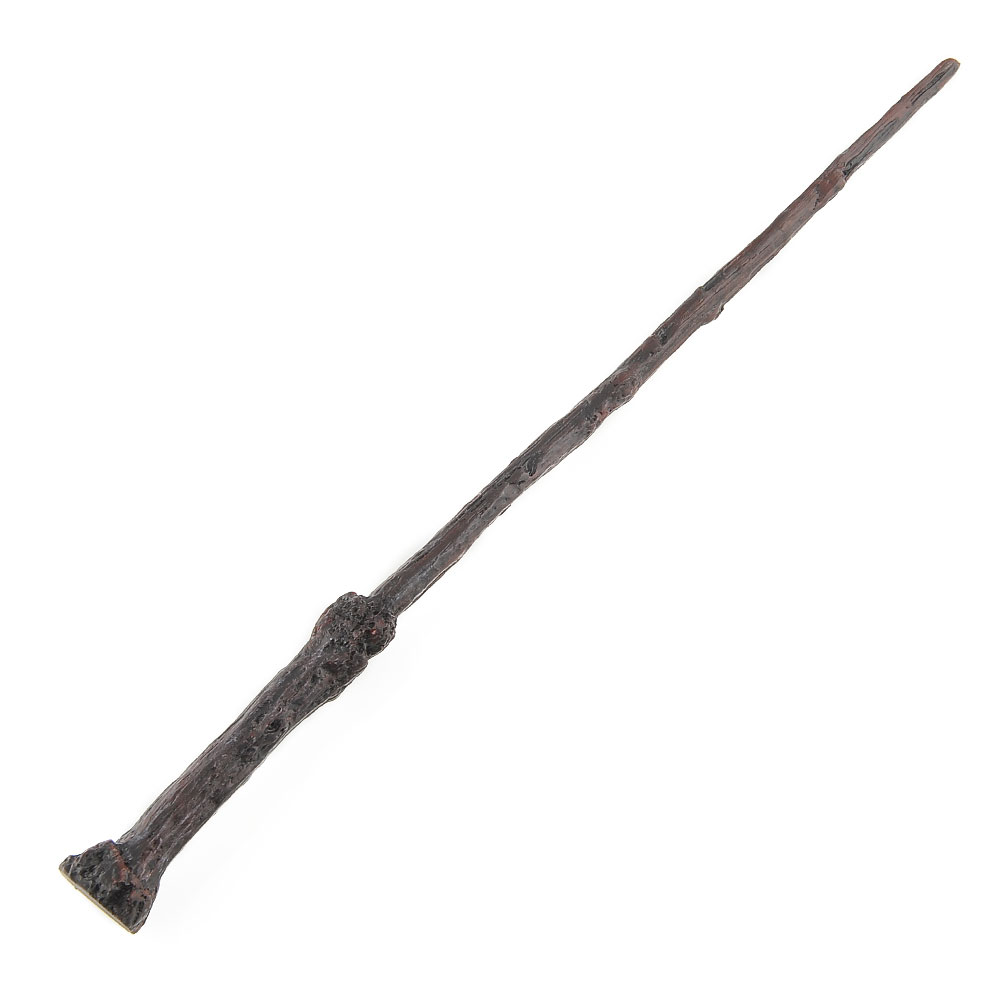
\includegraphics[scale=.03, angle = -20]{stick.jpg} }}

%нумерация глав
\renewcommand{\thesection}{Приложение  \Asbuk{section}} 

%этот кусок кода позволяет ссылаться на названия глав
\usepackage{nameref}
\makeatletter
\newcommand*{\currentname}{\@currentlabelname}




\begin{document}
\begin{titlepage}

\begin{figure}[h]
\vspace{-1cm}
\begin{center}

\includegraphics[height=6cm,keepaspectratio]{logo.png} 
\end{center}
\end{figure}

\vspace{1cm}

{\fontsize{12pt}{1}\selectfont Мистеру Виталику Олчею} 

\vspace{2.5cm}

Дорогой Виталий Олчей, \\

Приносим вам извинения за то, что это письмо пришло к вам только сейчас. Первая сова была убита темным магом, который напился и запускал в воздух смертельные заклинания. \\

Пожалуйста, ознакомьтесь с приложенным к данному письму списком необходимых книг и предметов.\\

Занятия начинаются 1 сентября. Ждем вашу электронную сову не позднее 31 июля.
\vfill
Искренне ваша,
\begin{figure}[H]

\includegraphics[scale=1]{signature}
\end{figure}
\vspace{-1cm}
Профессор Минерва МакГонагалл, заместитель директора Школы Чародейства и Волшебства «Хогвартс»
\begin{center}
\href{http://vhogwarts.ru}{{\fontsize{12pt}{1.33}\selectfont Школа Чародейства и Волшебства «Хогвартс»}}
\end{center}

\end{titlepage}

\section{Список необходимых книг и предметов}

\begin{itemize}
\item Волшебная палочка
\item Мантия невидимка
\item Шаурмичный корень (квадратный)
\item Экстракт пота
\item Сберегательная книжка
\end{itemize}
\newpage
\section{Список изучаемых предметов}

\begin{itemize}
\item Волшебный анализ
\item Линейная трансфигурация
\item Прорицание МНК
\item Нумерометрика
\item Дифференцальные руны (Дифф.руны)
\end{itemize}

\end{document}